\section{VizAPI Implementation}
\label{sec:implementation}
We now describe VizAPI, which includes two phases: (1) data extraction and (2) visualization. 

The data extraction phase uses static and dynamic
analysis to collect data about client usages of libraries. We generate both static and
dynamic call graphs, and we also capture other client-library interactions. The static analysis captures the
following interactions: vanilla invocations, field accesses, class usages,
setAccessible(), annotations and inheritance information. The dynamic
analysis captures all dynamic uses of those patterns and additionally
reflection, dynamic proxies and service loader bypasses.

The visualization phase transforms the data extracted in the first phase into d3 format by first converting the data into a graph and then using our customized version
of the d3graph\footnote{\url{https://pypi.org/project/d3graph/}} library in Python to generate d3js\footnote{\url{https://d3js.org/}} visualizations. 

In this section, we start by describing VizAPI. Next, we discuss its implementation. Then, in Section~\ref{sec:design-decisions}, we explore
alternatives that we could have chosen, including their advantages and
drawbacks.  The goal of this paper is to produce an explanation of our
artifact that will be helpful to other researchers, including in
particular an exploration of the design space for program analysis and visualization tools like ours.

\subsection{Overview}
We briefly give an overview of VizAPI to enable discussions of its design and implementation.
The VISSOFT paper~\cite{venkatanarayanan22:_vizap}
and the first author's MMath thesis~\cite{venkatanarayanan22:_study_lever_api_usage_patter} explain VizAPI in more detail.

We first define the terms ``client'', ``library'', ``dependency'' and ``interaction", which we use throughout this paper. A ``client'' is a software component which directly uses some functionality of an external component, which is the ``library''. Any external component that the ``library'' directly uses is a ``dependency'' of that library; components may also have ``transitive dependencies''. The pattern observed when a client/library boundary is crossed is an ``interaction". 

VizAPI creates graphs where the nodes are packages that belong to components (clients, libraries and dependencies) and the edges represent the types of interactions between the packages. We create these graphs with the goal of being useful to developers who are thinking about API design questions for their clients and libraries.

\begin{figure}[h]
\begin{center}
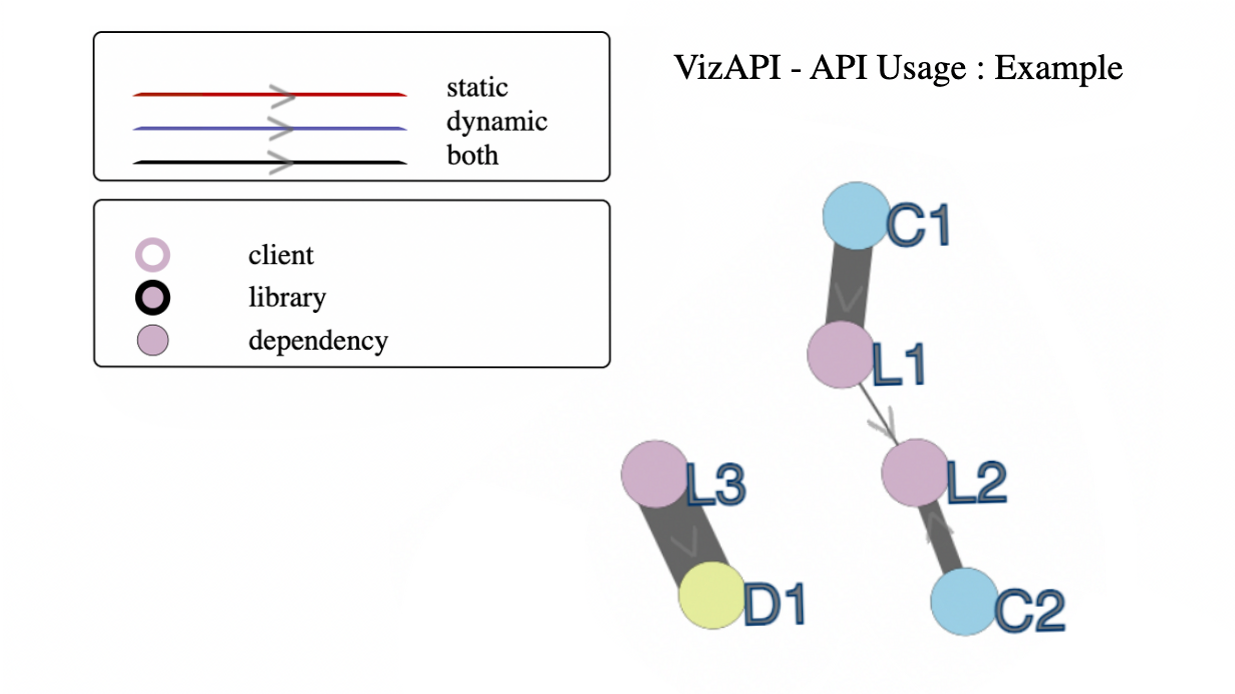
\includegraphics[height=4cm,width=7cm]{images/intro-example.png}
\caption{VizAPI visualization of client C which calls library L, itself dependent on dependency D.}
\label{fig:example}
\end{center}
\end{figure}

Figure~\ref{fig:example} illustrates a VizAPI usage scenario, from the perspective of a client developer worried about breaking changes from a new version of a library. It shows Java client $C$ (blue nodes) and library $L$ (purple nodes). Library $L$ has packages $L_1$, $L_2$, and $L_3$. $C$ calls into $L_1$ and $L_2$. Internally, within $L$, $L_1$ and $L_2$ call into each other, but not into $L_3$. The VizAPI result, with no edges from $C$ directly to $L_3$, allows a developer to conclude that breaking changes in $L_3$ will not affect $C$. Also, if only $L_3$ uses an external dependency $D$ (yellow node), then $C$ will not need $D$ to be on its classpath.

To produce its graphs, VizAPI needs to collect information about interactions between clients, libraries, and dependencies. We provide a few examples of interactions---enough to give the idea of what VizAPI is looking for, but not an exhaustive list.

\paragraph{Vanilla invocations} The goal here is to capture information about straightforward (``vanilla'') method calls between components, in opposition to the more complicated interactions discussed immediately below. This information can be approximated statically using Class Hierarchy Analysis, as we describe below. Furthermore, it can also be captured precisely at runtime, at least for the invocations that happens on a particular set of executions.

\paragraph{Dynamic proxies and reflective calls} We use a dynamic approach for recording calls made using Java dynamic proxies and Java reflection to avoid needing to make hopelessly conservative approximations. The soundiness manifesto~\cite{livshits15:_in_defen_sound} points out that many papers in the literature claim soundness and are, in fact, sound for most language features, but exclude highly dynamic features like reflection. VizAPI uses dynamic information and instrumentation to capture certain patterns of reflection and dynamic proxies.

\paragraph{Service Loaders} This Java API allows Java programs to dynamically load additional code, typically plugins. The plugins would declare a published interface, which we can record statically. VizAPI captures uses of the published interface as well as dynamic calls that exceed the public interface.


\subsection{Overall Design of VizAPI}
We now explain the design of our VizAPI tool, which integrates data from both static and dynamic analysis.
We use Javassist~\cite{chiba00:_load_struc_reflec_java} for our static analysis, which we discuss in Section~\ref{subsec:static}. We also use Javassist to instrument the code so that we can
collect dynamic analysis data; we discuss that part in
Section~\ref{subsec:dynamic}.

Our static and dynamic analysis tool takes in a set of clients and libraries as input.
We programatically obtain a list of dependencies for each client and library by invoking Maven, and locate the JARs that Maven downloads in its build output.
We first record the extents of components (clients, libraries, and dependencies) by inspecting JAR
files of each software component to obtain a
list of classes for that component. We associate classes and their
members to components based on these lists.  This allows us to
identify interactions across the client/library boundaries (i.e. between classes that appear on different lists).
Using Maven, we build JAR
files that contain source code only. This ensures that we do not
capture library uses meant solely for unit testing. 

Figure~\ref{fig:workflow} summarizes our
(static) data capture and (dynamic) instrumentation workflow.  \\

\begin{figure*}[h]
 \begin{center}
\resizebox{0.9\textwidth}{!}{
  \begin{tikzpicture}
    \node[block] (client) {client};
    \node[block,below=1cm of client] (library) {library};

    \draw (library) -- node[left] (depends) {depends on} (client);

    \node[above left=.75em of client] (ja) {\begin{minipage}{7em} modify \\with Javassist \end{minipage}};
    \draw[-Latex] (ja) -> (client);
    \draw[-Latex] (ja) to [->,bend right=35] (library.west);

    \node[block, above right=2em of client,xshift=-2em] (olib) {other library};
    \draw (client) -- node[right,xshift=.1em] (also) {also depends on} (olib);

    \node[oval,right=of depends] (test) {maven: run tests};

    \draw[-Latex] (client) to [->,bend left=15] (test);

    \node[block, right=10em of client] (output) {test output};
    \node[block, right=10em of library] (raw) {raw API usage info};

    \draw[-Latex] (test) to (output);
    \draw[-Latex] (test) to (raw);

    \node[oval, right=of raw] (Py) {Python scripts};
    \draw[-Latex] (raw) to (Py);

    \node[block, right=1em of Py] (viz) {D3 visualizations};
    \draw[-Latex] (Py) to (viz);
  \end{tikzpicture}
}
  \caption{Our instrumentation workflow. Using Javassist, we analyze and instrument clients and run their test suites. (We process the generated data with Python scripts to create D3 visualizations for VizAPI.)}
  \label{fig:workflow}
 \end{center}
\end{figure*}



\subsection{Static Analysis}
\label{subsec:static}
It turns out that a simple (rather straightforward) static analysis suffices
for our purposes, and we describe parts of it in this section. Section~\ref{sec:design-decisions}
discusses when the use of more sophisticated analyses is appropriate, and
how to incorporate such analyses in an analysis pipeline.

For VizAPI, using Javassist, we 
perform class hierarchy analysis on components and create a static call
graph. 

We implement class hierarchy analysis ourselves. We first read the class files from JARs of clients, libraries, and dependencies (provided by Maven) and we record
inheritance relationships between classes. Then, when we walk through the different kinds of interactions,
 we add an edge between the caller and its potential callees---because we use Class Hierarchy Analysis, the set of potential callees follows from the recorded inheritance relationships.
Some of the interactions we record include vanilla invocations, subtyping and annotations.

\paragraph{Vanilla invocations}
The standard case is simple. At every invoke instruction in every
loaded method which transfers control between a client and a
library, we record a static dependency using the class hierarchy
analysis call graph that we compute.

\paragraph{Subtyping}
We record information about all superclasses and implemented interfaces that cross the library/client barrier. 

\paragraph{Annotations}
We have a quasi-static approach for finding class, field and method annotations:
we observe all annotations for a class or class member when it is loaded, and
record cases where a class or member declares an annotation from the library of interest.

\subsection{Dynamic Analysis}
\label{subsec:dynamic}
We collect dynamic data about client usages of libraries by running client
test suites under instrumentation. The instrumentation records API
uses which cross client/library boundaries, closely mirroring the API
usage patterns
in~\cite{venkatanarayanan22:_study_lever_api_usage_patter}. We first
describe how we capture specific dynamic interactions between components, and
then discuss our instrumentation implementation.

\paragraph{Vanilla invocations} 
At every invoke instruction in every
loaded method which transfers control between a client and a
library, we add code to dynamically record
the invoke by incrementing a counter just before the invoke
executes. Note that we handle all Java invocation types, including
virtual and even dynamic invokes. Crossing the client/library boundary
includes conventional calls from the client to the library as well as
callbacks from the library to the client.  Because we instrument
libraries, we can record both invocation directions.

\paragraph{Dynamic proxies and reflective calls}
Our instrumentation intercepts calls to
\texttt{java.lang.reflect.Method.invoke()}, a distinguished method
used to invoke dynamic proxies and reflective calls, 
recording details of the calls that we intercept at runtime. It is possible for
static analyses to resolve a subset of such calls using clever
techniques~\cite{christensen03:_precis_analy_strin_expres}. Our static analysis machinery does not provide enough information to
statically resolve this dependency, but we have full visibility on
calls that actually happen dynamically.

\paragraph{Service Loaders} Before the instrumentation, we record a list 
of services and their implementations by statically inspecting files in \texttt{src/main/resources/META-INF/services}. 
This gives a static list of dependencies; anything beyond this list that we observe dynamically would be a service bypass. 
In the dynamic phase, we use the statically recorded information to dynamically detect service bypasses which are direct uses of service implementation 
classes in clients, either through instantiations, casts or reflection. To do so, we intercept calls 
to method \texttt{load()} in classes with name \texttt{Service*Loader} and record any calls to methods beyond 
the published interface that we have recorded statically.

\paragraph{How we implemented instrumentation}
In the dynamic analysis phase, we modify the build system of each
client (we chose clients that all use Maven) to run its provided unit tests on instrumented code.
Asking the modified build system to run the client's tests gives us dynamic call graphs as a side-effect output.

Specifically, using the Java instrumentation APIs and getting them to call Javassist APIs that modify bytecode,
we instrument classes and their members to increment counters for every interaction source
with a destination lying outside the JAR that it belongs to.
Our system creates code to carry out instrumentation and places it into a Java agent JAR.
The agent is then passed as an argument to Maven when running client unit tests, which attaches it to the JVM.
Once classes are loaded, the agent modifies the bytecode and it is then executed.
The code that we insert during the instrumentation phase keeps track of interactions and counters,
and writes them out upon program termination. \\


While our current benchmark set consists of 101 projects, it is possible to run both our static and dynamic analysis tool and the VizAPI visualization tool on new libraries and clients. However, when a library developer wishes to use VizAPI, they are required to provide a specific set of clients that they wish to observe as input to the tools. Developers can use libraries.io to find popular clients of libraries---it provides a dependency tree based on projects' packaging information.


\subsection{Visualizations}
\label{subsec:vis-system}

\begin{figure*}[h]
\begin{center}

\subfloat[Usage Scenario 1: Library \textit{jsoup} (pink with dark borders), called by two clients, \textit{ez-vcard} (hollow with purple border) and \textit{JsoupXpath} (hollow with pink border). Exploration shows that internal jsoup packages aren't called directly by clients.
\label{fig:usagescenario1}]
{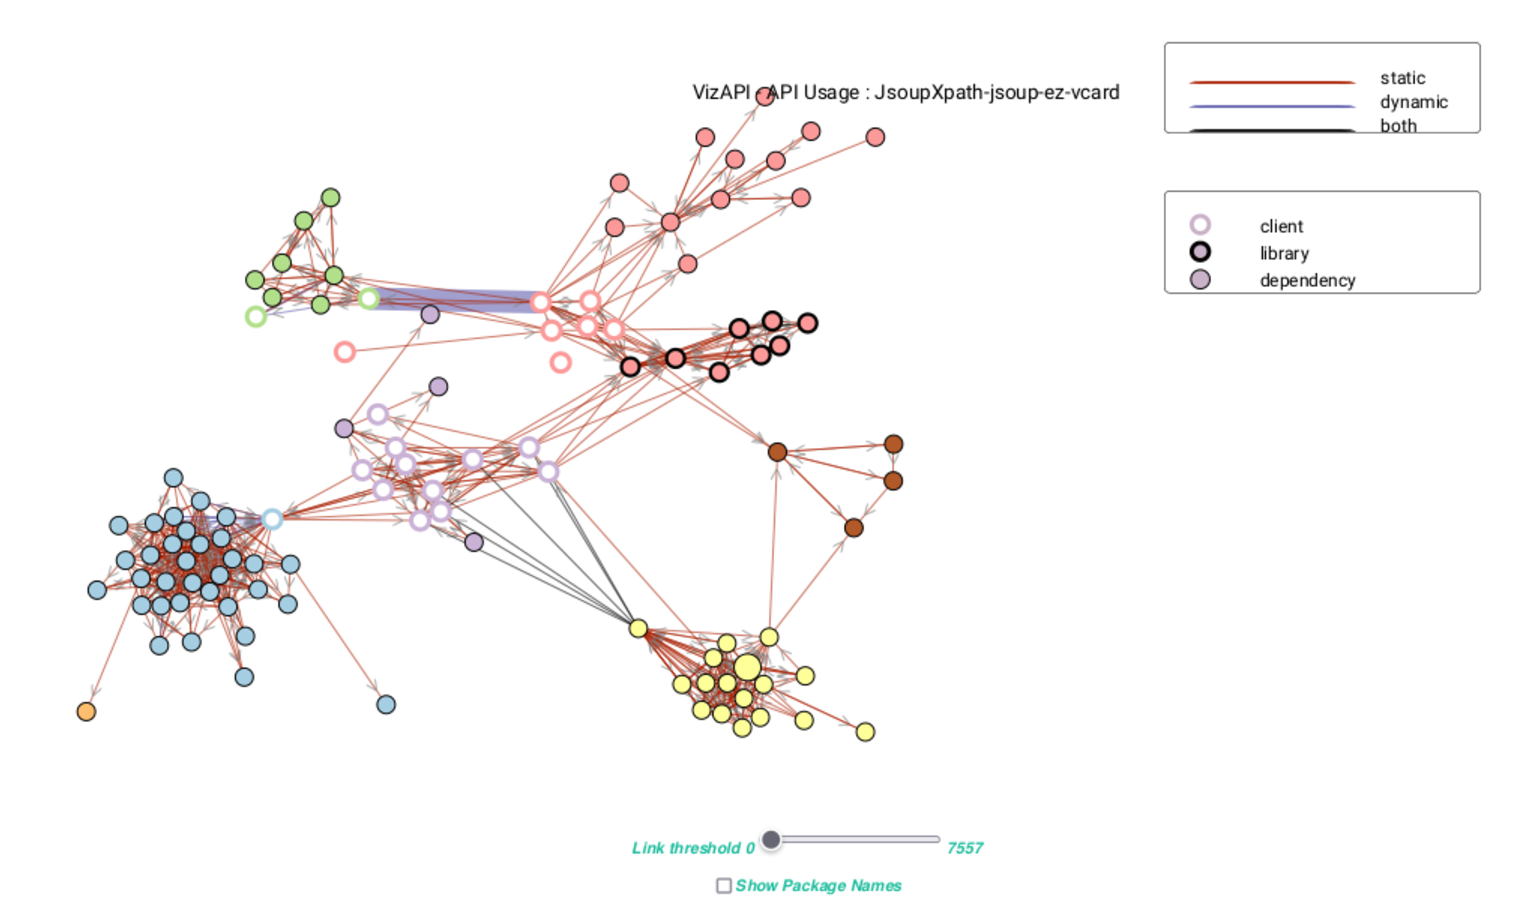
\includegraphics[width=16cm]{images/usage-scenario1.pdf}}
\hspace{7mm}

\subfloat[Usage Scenario 2: Client \textit{dataprocessor} (hollow, orange border) calls only one package in library \textit{fastjson} (green fill).
\label{fig:usagescenario2}]
{
\makebox[16cm]{
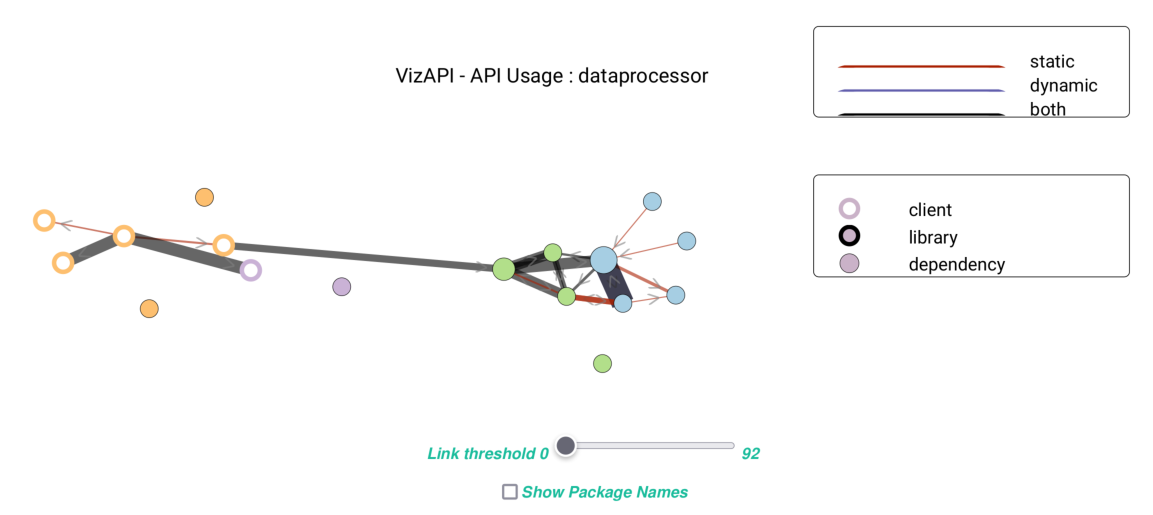
\includegraphics[width=11cm]{images/usage-scenario2.pdf}
}
}
\caption{\label{fig:usagescenarios} VizAPI Usage Scenarios.}

\end{center}
\end{figure*}


Once we have generated static and dynamic analysis data using our tool, we use a modified version
of the d3graph\footnote{\url{https://pypi.org/project/d3graph/}} library in Python to generate a d3js\footnote{\url{https://d3js.org/}}
visualization. The modifications that we made to the d3graph  library in Python include styling changes (for example, changing node styles based on whether it is a client, library or dependency),
legends, and a toggle to show all package names. 
The graphs in Figures~\ref{fig:example}, \ref{fig:usagescenario1}, and \ref{fig:usagescenario2} are examples of graphs produced by VizAPI.

VizAPI graphs are force-directed graphs based on the frequency of
interactions between different software components. 
Here, frequency of interactions indicates the sum of number of times different kinds of interactions occur.
Each node is a
set of one or more packages that belong to the same JAR.  There are
three categories of nodes: clients are represented by nodes with white
interiors; libraries by nodes with filled interiors and black borders;
and dependencies (called by libraries but not clients) by nodes with
filled interiors and normal borders.  We coalesce nodes if they
originate from the same JAR and have the same incoming and
outgoing edges.

Each edge is directed
from the source package(s) to the target package(s) and represents an interaction 
(e.g. invocations, fields, annotations, subtyping) between packages. 
The thickness of each edge reflects the frequency of interactions between the source and the target.
Double-clicking on a node emphasizes its direct interactions with other packages while fading out the rest of the graph.
To search for a package, the user can click on ``show package
names'' and use the browser’s find functionality. 
The ``Link threshold'' slider allows the user to form new clusters based on frequencies of interactions.


We run a Python implementation of the Louvain clustering algorithm~\cite{blondel2008fast}, and make the clusters 
visible by colouring nodes based on cluster.
Nodes of the same cluster may come from the same or different JARs.
Hovering on a node shows the list of packages and 
the JAR that they belong to, 
formatted as ``jar : $\langle$space separated list of packages$\rangle$''. 
Hovering on an edge shows the type of interaction (invocations, fields, annotations, subtyping or a combination of these) between nodes.
